\section{K-nearest neighbors}

% ----- Q.1 ----- %
\subsection{Effect of the number of neighbors on the decision boundary}

% ----- Q.1.a
\subsubsection{{\it Illustrate the decision boundary for each number of neighbors}}
We built several k-NN models with different numbers of neighbors, for both datasets. To illustrate our results, we present the decision boundary of each model at figures \ref{fig:knn_make_data1} (for dataset 1) and \ref{fig:knn_make_data2} (for dataset 2).\par
In order to make the visualization clearer, we only displayed \num{25}\% of the points of each testing set and only decided to show the most interesting plots, the other being easily interpolated from the graphs shown.
\begin{figure}[H]
    \centering
    \begin{subfigure}{0.495\textwidth}
        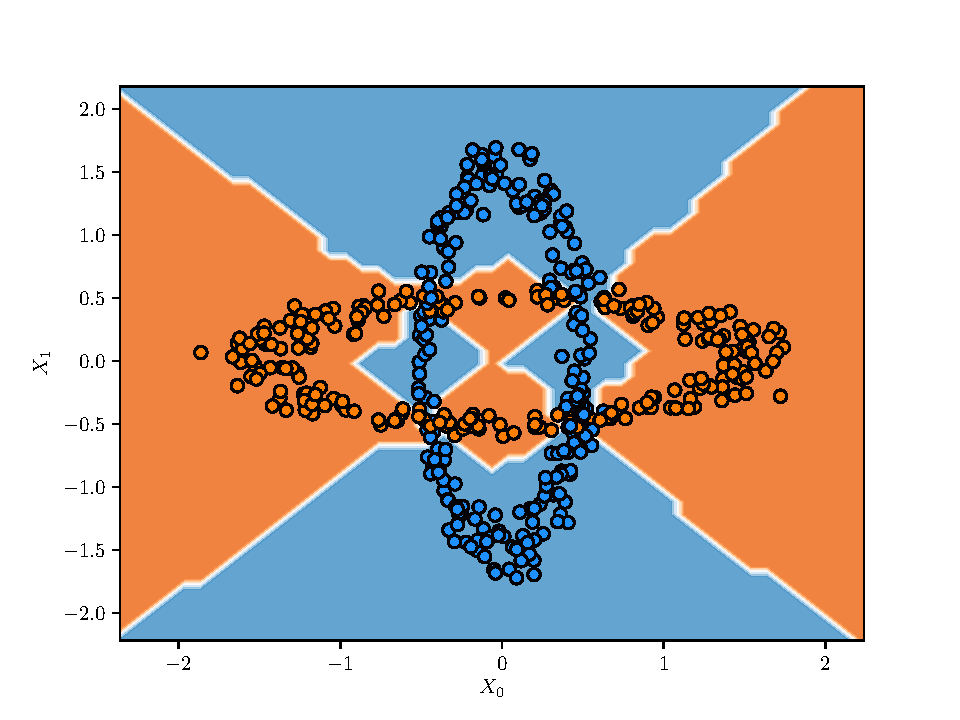
\includegraphics[width=\textwidth]{resources/pdf/make_data1_knn_1.pdf}
        \caption{k-NN : 1 neighbor (acc = \num{0.94})}
    \end{subfigure}
    \begin{subfigure}{0.495\textwidth}
        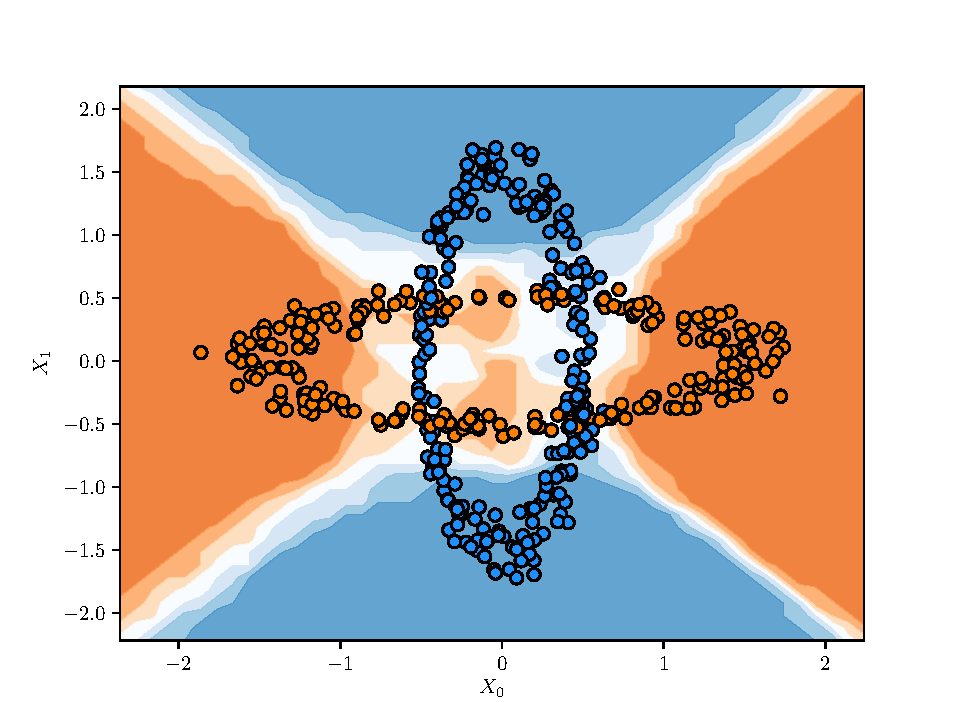
\includegraphics[width=\textwidth]{resources/pdf/make_data1_knn_10.pdf}
        \caption{k-NN : 10 neighbors (acc = \num{0.86})}
    \end{subfigure}
    \vspace{3pt}
    \begin{subfigure}{0.495\textwidth}
        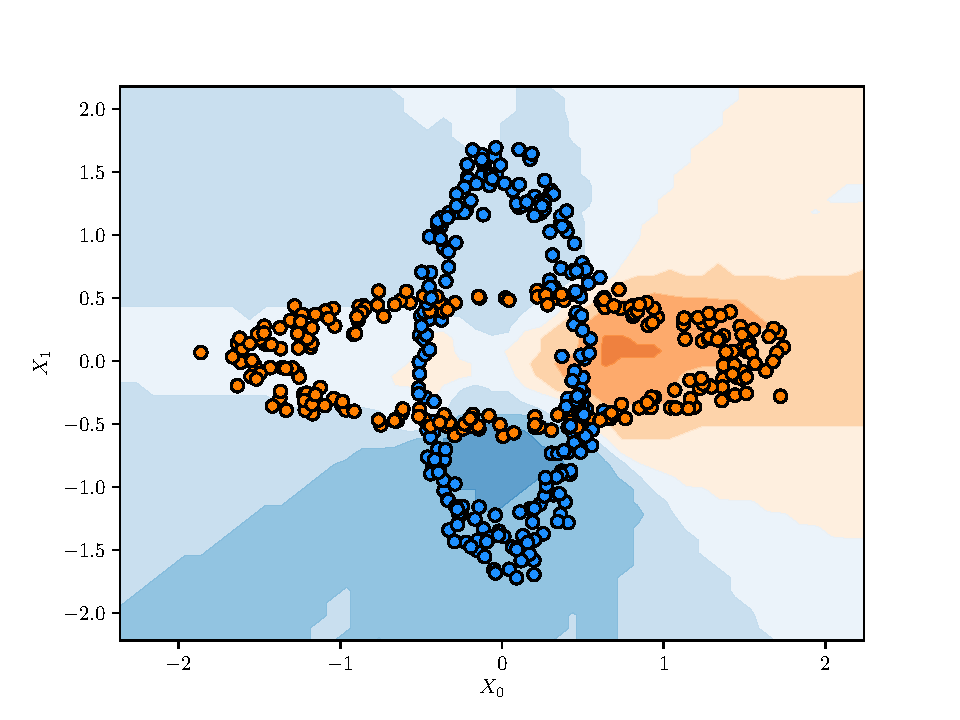
\includegraphics[width=\textwidth]{resources/pdf/make_data1_knn_75.pdf}
        \caption{k-NN : 75 neighbors (acc = \num{0.75})}
    \end{subfigure}
    \begin{subfigure}{0.495\textwidth}
        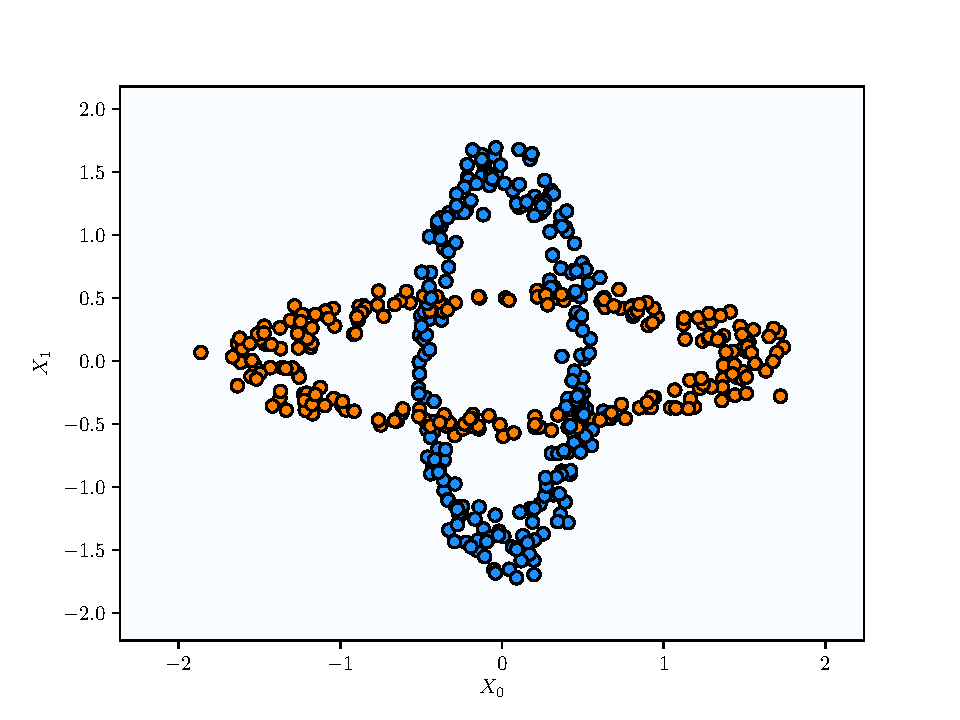
\includegraphics[width=\textwidth]{resources/pdf/make_data1_knn_150.pdf}
        \caption{k-NN : 150 neighbors (acc = \num{0.5})}
    \end{subfigure}
    \noskipcaption{k-NN boundary for several number of neighbors using \texttt{make\_data1}}
    \label{fig:knn_make_data1}
\end{figure}
\begin{figure}[H]
    \centering
    \begin{subfigure}{0.495\textwidth}
        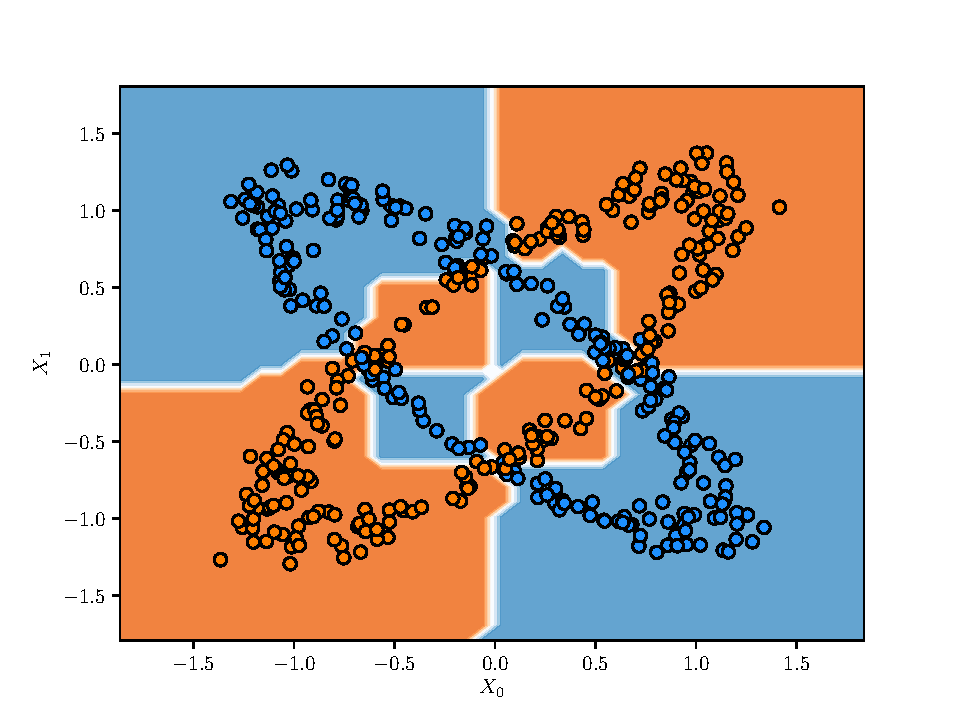
\includegraphics[width=\textwidth]{resources/pdf/make_data2_knn_1.pdf}
        \caption{k-NN : 1 neighbor (acc = \num{0.94})}
    \end{subfigure}
    \begin{subfigure}{0.495\textwidth}
        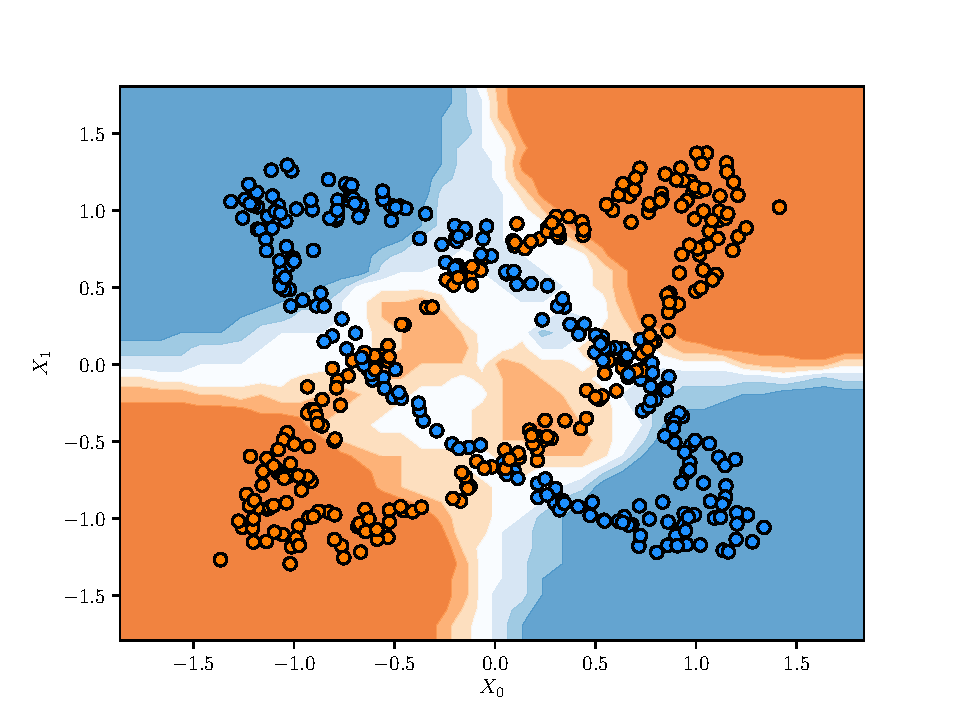
\includegraphics[width=\textwidth]{resources/pdf/make_data2_knn_10.pdf}
        \caption{k-NN : 10 neighbors (acc = \num{0.86})}
    \end{subfigure}
    \vspace{3pt}
    \begin{subfigure}{0.495\textwidth}
        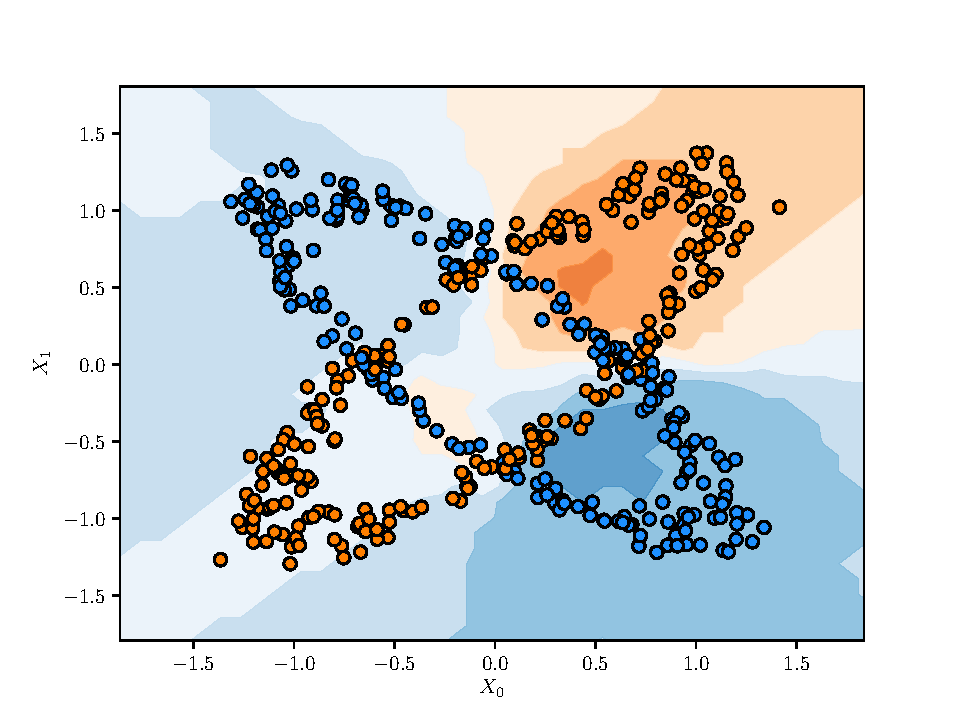
\includegraphics[width=\textwidth]{resources/pdf/make_data2_knn_75.pdf}
        \caption{k-NN : 75 neighbors (acc = \num{0.75})}
    \end{subfigure}
    \begin{subfigure}{0.495\textwidth}
        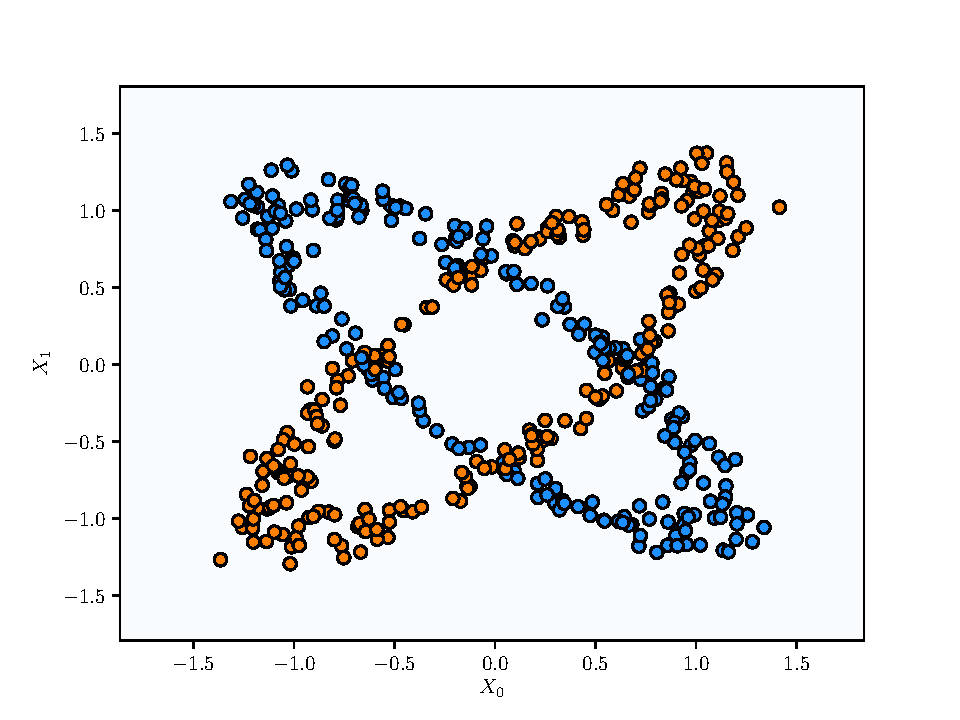
\includegraphics[width=\textwidth]{resources/pdf/make_data2_knn_150.pdf}
        \caption{k-NN : 150 neighbors (acc = \num{0.5})}
    \end{subfigure}
    \noskipcaption{k-NN boundary for several number of neighbors using \texttt{make\_data2}}
    \label{fig:knn_make_data2}
\end{figure}

% ----- Q.1.b
\subsubsection{{\it Evolution of the decision boundary with respect to the number of neighbors}}
The more neighbors, the less confident the algorithm seems to be about what to classify the sample. It is easily understood as, for one neighbor, the certainty of being \og{}right\fg{} is of \num{100}\%, whereas, for a greater number of neighbors, \num{100} for example, the probability can easily reduce as low as \num{50}\% depending on the position of the sample. That is represented by a decision boundary of a pale color. The more neighbors, the more uncorrelated data you take into account in your decision (they are far away from the sample position and should not have a great influence on the decision).\par
For \num{150} neighbors, all the space is whitish as there are almost as many points from the dataset 1 as from the dataset 2 in the learning sample used to establish the probabilities (there are a bit more blue points, which makes the boundary slightly bluish). Every testing sample will therefore have the same neighbors (the training sample is composed of 150 points), and so the whole space has a uniform decision boundary.\par
The paler the color, the more uncertain the model is about its prediction. As the two datasets show two \og{}symmetric\fg{} axes (some sort of diagonals), these are white from the start, and expand as the number of neighbors increases.\par
In both cases, for a small number of neighbors (1 and 10), the classifications seem correct but quite too specific (1 neighbor is a case of overfitting, 10 neighbors is smoother). For a larger number of neighbors (75 or more), the classification is degraded (case of underfitting) : the high number of neighbors allows the algorithm to use a larger series of points irrelevant for the zone, thus distorting the probabilities.

% ----- Q.2 ----- %
\subsection{Ten-fold cross validation}

% ----- Q.2.a
\subsubsection{{\it Explain your methodology}}
This technique consists in sampling our whole dataset in \num{10} samples. One sample is chosen as the testing set and the other \num{9} are used at learning sets.\par
The score (accuracy) is then computed and the operation is repeated by taking another testing set among the samples not yet used as such.\par
The operation is therefore repeated \num{9} times so that each sample is used once as testing set. The \num{10} computed scores are averaged to obtain the score for that number of neighbors.\par
As part of our project, we used the function \texttt{cross\_val\_score} of the \texttt{sklearn} library : it returns a scoreboard that contains the score of each of the 10 subsets. We computed the mean of this scoreboard in order to have the score of this strategy. That score was then used to find the optimal number of neighbors, as described below. The estimate is unbiased because it does not depend anymore on $150$ specific samples, but takes into account the whole dataset.

% ----- Q.2.b
\subsubsection{{\it Score and optimal number of neighbors to use}}
To determine the optimal number of neighbors to use, we tested the ten-fold cross validation strategy on several number of neighbors (from \num{5} to \num{150} with a step of 1) and computed the score for each. These scores are shown in figure \ref{fig:knn_score}.
\begin{figure}[H]
    \centering
    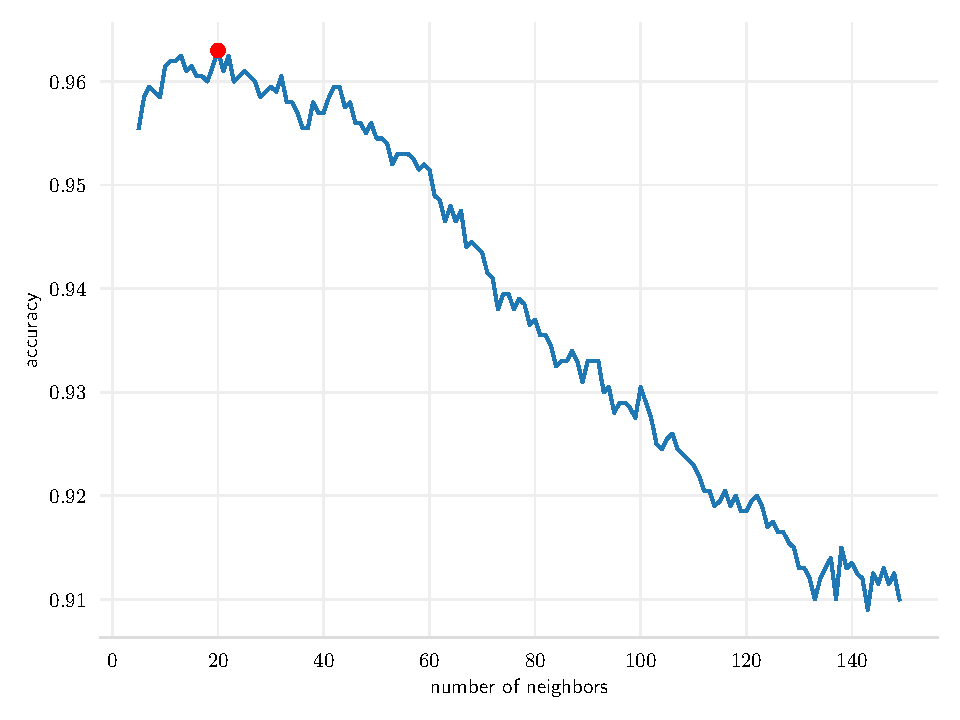
\includegraphics[width=0.9\textwidth]{resources/pdf/knn_kfold_scores.pdf}
    \caption{Scores obtained for multiple value of number of neighbors with k-fold strategy on dataset 2}
    \label{fig:knn_score}
\end{figure}
The scores obtained show us that the optimal number of neighbors to take is \num{20}. This number provides an accuracy of \num{0.963}.\par
This result is in agreement with our intuition : an optimal number of neighbors is not very high so as not to take into account too many specific or isolated points but is not too small so that the decision is not dictated by a very small group of points that could be noise or make the strategy local, blind to the bigger picture.\par
The decision boundaries also confirm this intuition : as seen on figure \ref{fig:knn_make_data2}, the optimal value was between \num{1} (underfitting) and \num{75} (overfitting).\par
\paragraph{NB :} It is worth noting that the k-cross test validation was performed on the whole dataset (2000 samples), and not on the 150 training samples alone. This explains why the accuracies given in this section are much higher than the ones given in the plots of the first section.

% ----- Q.3 ----- %
\subsection{Optimal value on the first dataset}
We believe it would fare almost in the same way as it did for the second dataset, as the ellipse dispositions are almost the same in each dataset, and as k-NN is rotational invariant. Indeed, the distance between 2 objects is rotational invariant.\par
To confirm our hypothesis, we made the test for the first dataset and found out that, indeed, 20 neighbors is optimal.
